\documentclass[11pt,a4paper]{article}
\usepackage[utf8]{inputenc}
\usepackage[T1]{fontenc}
\usepackage[margin=22mm]{geometry}
\usepackage{array}
\usepackage{longtable}
\usepackage{hyperref}
\usepackage{xcolor}
\usepackage{tikz}
\usetikzlibrary{arrows.meta,positioning}

\title{HyMeKo platform strategy and execution plan}
\author{Strategy ID: HYMEKO-PLATFORM-2026-09-01-v1}
\date{2026-09-01}

\begin{document}
\maketitle

\section{Objective}
Build one high-performance, memory-efficient, parallel, hypergraph-native
platform around \texttt{hymeko\_core::ir::Ir}. Parser, graph algorithms,
tensor/HNN, WebXR, distributed updates and MCU endpoints consume the same
semantics. Derived structures are exact sparse indexes or numerical projections,
never independent models.

\section{Binding principles}
\begin{enumerate}
  \item One canonical mutable Ir; no Editor-IR or endpoint DTO as authority.
  \item Direct hypergraph navigation through exact \texttt{(HyperArcId, slot)}
        incidence coordinates.
  \item Star is the sparse operator $B$; use $Bx$, $B^Ty$ and $B^TBx$.
  \item No default clique/2-section materialisation.
  \item One sectioned \texttt{ir\_stream} wire format for distribution and MCU.
  \item Transactions are atomic; readers observe immutable versioned snapshots.
  \item One downstream product CLI; libraries remain the tested API surface.
\end{enumerate}

\section{Measured constraints}
At one million incidences, $Bx$ is 5.2--5.9 ms, $B^Ty$ is 17.6--28.9 ms and
$B^TBx$ is 22.8--35.3 ms on the 2026-09-01 quiet-host survey. Direct-Ir walks
are provisionally 13--17 ns/incidence. WebXR validation is linear at about
0.31 microseconds/entity. The exact reverse index retains 12.4--14.8
bytes/incidence. A generational arena is deferred: its best prototype regressed
valid lookup by 56 percent versus the append-only dense record table.

\section{Roadmap}
\begin{longtable}{>{\bfseries}p{10mm} p{35mm} p{94mm}}
P0 & Evidence consolidation & Verify refs, ancestry and full gates; no silent merge.\\
P1 & Benchmark consolidation & One owner per generator, oracle and workload; preserve all KATs.\\
P2 & Incidence precompute & Improve $B^Ty$ locality while preserving exact coordinates, weights and FP order.\\
P3 & Direct-Ir locality & Improve sparse traversal and measured Rayon thresholds without a second graph model.\\
P4 & Mutable storage study & Compare deletion-capable ID/storage candidates under identical churn.\\
P5 & Transactions & Native atomic delta API; no partial commit; value/topology paths separated.\\
P6 & Snapshots and refresh & Lock-free readers, versioned sparse index, incremental non-topology refresh.\\
P7 & Distributed apply & Idempotence, conflict/gap recovery and replica convergence over ir\_stream.\\
P8 & MCU C PoW & Same frozen bytes in Rust/C11, zero heap, malformed corpus, ASan/UBSan.\\
P9 & WebXR query & Borrowed canonical-ID queries; durable events return through transactions.\\
P10 & Accelerators & Sparse $B/B^T$ on WGPU, CUDA control and FPGA streaming boundary.\\
P11 & Single CLI & Downstream facade after stable library surfaces; no dependency cycle.\\
\end{longtable}

\section{Acceptance contract}
Every production phase requires positive, negative, metamorphic and independent
oracle tests; small/medium/large workloads; workspace and touched-line coverage;
cold/prepared/resident/end-to-end timing separation; allocation and retained
memory reporting; A/A null measurements; ownership and duplication audit; exact
commit/ref verification. Core edits require their own approval token.

\section{Prompt reference}
Future tasks cite:
\begin{verbatim}
GOVERNING-STRATEGY: docs/hymeko-platform-strategy.md
STRATEGY-ID: HYMEKO-PLATFORM-2026-09-01-v1
ROADMAP-TASK: P<n> / <slug>
\end{verbatim}
The full normative text is in \texttt{docs/hymeko-platform-strategy.md}.

\section{Architecture figure}
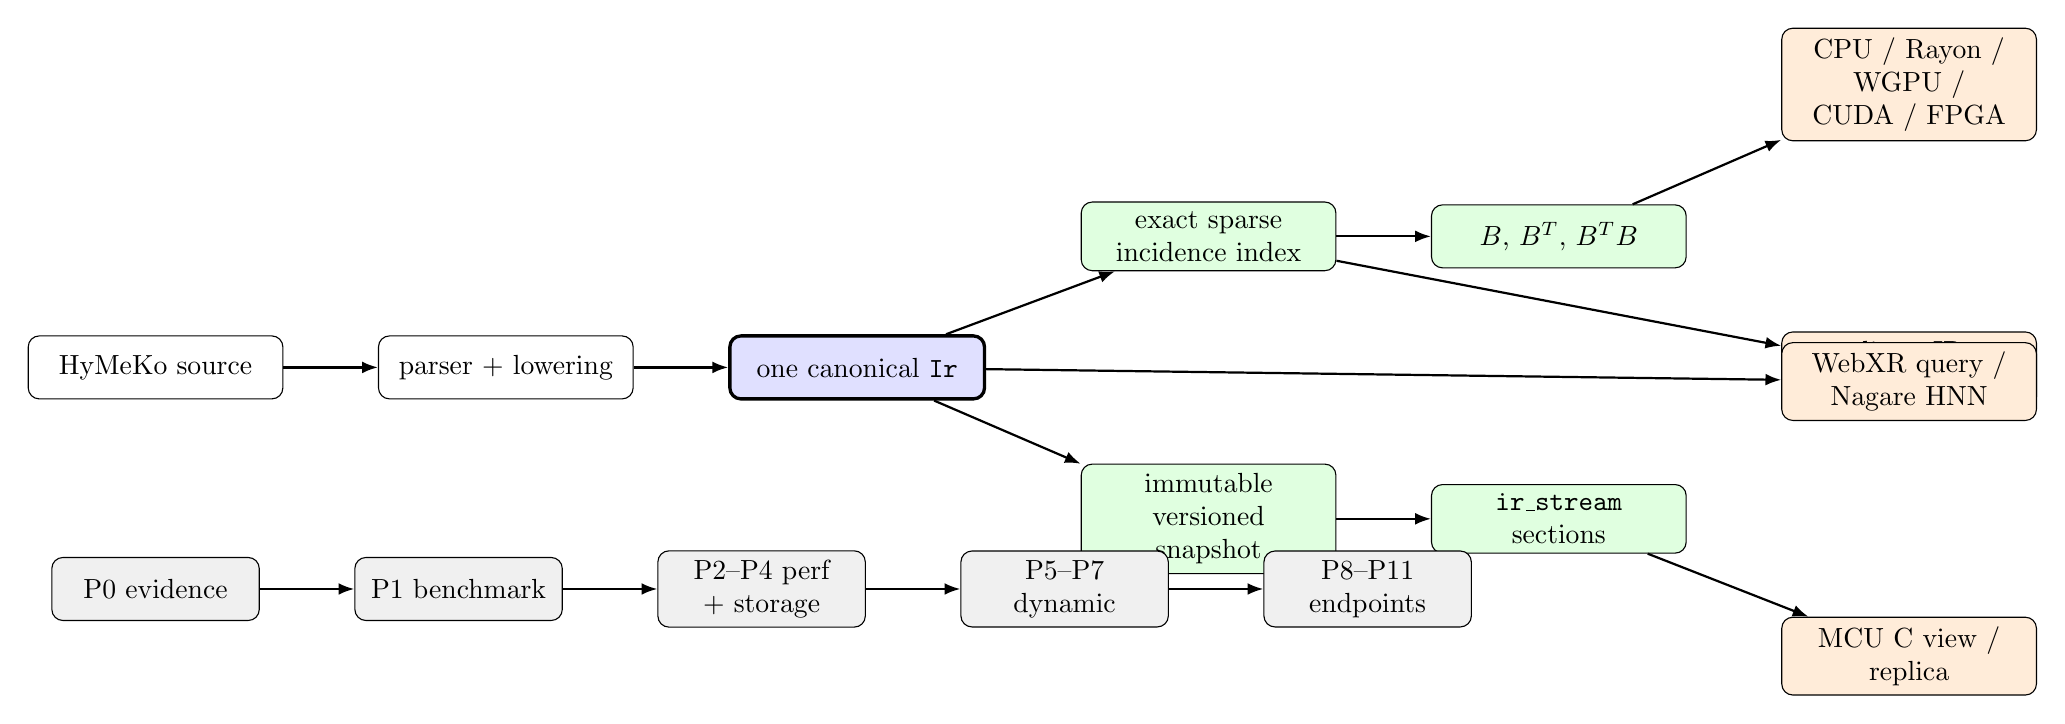
\begin{tikzpicture}[
  node distance=8mm and 12mm,
  box/.style={draw, rounded corners, align=center, minimum height=8mm, text width=30mm},
  core/.style={box, fill=blue!12, very thick},
  derived/.style={box, fill=green!12},
  endpoint/.style={box, fill=orange!15},
  phase/.style={box, fill=gray!12, text width=24mm},
  arrow/.style={-{Latex[length=2mm]}, thick}
]
\node[box] (source) {HyMeKo source};
\node[box, right=of source] (parser) {parser + lowering};
\node[core, right=of parser] (ir) {one canonical \texttt{Ir}};
\node[derived, above right=of ir] (inc) {exact sparse\\incidence index};
\node[derived, right=of inc] (ops) {$B$, $B^T$, $B^TB$};
\node[endpoint, above right=of ops] (compute) {CPU / Rayon /\\WGPU / CUDA / FPGA};
\node[endpoint, below right=of ops] (graph) {direct-IR\\graph algorithms};
\node[derived, below right=of ir] (snapshot) {immutable versioned\\snapshot};
\node[derived, right=of snapshot] (stream) {\texttt{ir\_stream}\\sections};
\node[endpoint, below right=of stream] (mcu) {MCU C view /\\replica};
\node[endpoint, above right=of stream] (webxr) {WebXR query /\\Nagare HNN};

\draw[arrow] (source) -- (parser);
\draw[arrow] (parser) -- (ir);
\draw[arrow] (ir) -- (inc);
\draw[arrow] (inc) -- (ops);
\draw[arrow] (ops) -- (compute);
\draw[arrow] (inc) -- (graph);
\draw[arrow] (ir) -- (snapshot);
\draw[arrow] (snapshot) -- (stream);
\draw[arrow] (stream) -- (mcu);
\draw[arrow] (ir) -- (webxr);

\node[phase, below=20mm of source] (p0) {P0 evidence};
\node[phase, right=of p0] (p1) {P1 benchmark};
\node[phase, right=of p1] (p24) {P2--P4 perf + storage};
\node[phase, right=of p24] (p57) {P5--P7 dynamic};
\node[phase, right=of p57] (p811) {P8--P11 endpoints};
\draw[arrow] (p0) -- (p1);
\draw[arrow] (p1) -- (p24);
\draw[arrow] (p24) -- (p57);
\draw[arrow] (p57) -- (p811);
\end{tikzpicture}


\end{document}
